%%
%%

\section*{Customizing the Configuration Files}
\label{_ChapterStart16}
\index[general]{Files!Customizing the Configuration }
\index[general]{Customizing the Configuration Files }
\addcontentsline{toc}{section}{Customizing the Configuration Files}

When each of the Bacula programs starts, it reads a configuration file
specified on the command line or the default {\bf bacula-dir.conf}, {\bf
bacula-fd.conf}, {\bf bacula-sd.conf}, or {\bf console.conf} for the Director
daemon, the File daemon, the Storage daemon, and the Console program
respectively. 

Each service (Director, Client, Storage, Console) has its own configuration
file containing a set of Resource definitions. These resources are very
similar from one service to another, but may contain different directives
(records) depending on the service. For example, in the Director's resource
file, the {\bf Director} resource defines the name of the Director, a number
of global Director parameters and his password. In the File daemon
configuration file, the {\bf Director} resource specifies which Directors are
permitted to use the File daemon. 

Before running Bacula for the first time, you must customize the configuration
files for each daemon. Default configuration files will have been created by
the installation process, but you will need to modify them to correspond to
your system. An overall view of the resources can be seen in the following: 

\addcontentsline{lof}{figure}{Bacula Objects}
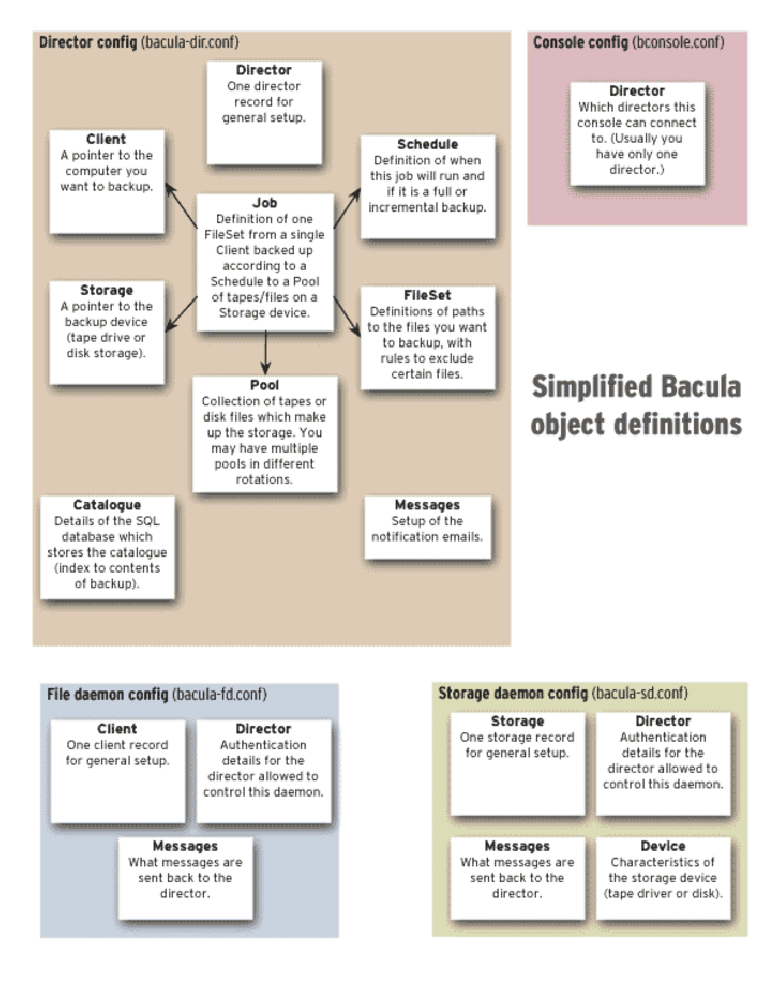
\includegraphics{./bacula-objects.eps} 
\\
(thanks to Aristedes Maniatis for the above graphic) 
\label{ResFormat}

\subsection*{Resource Directive Format}
\index[general]{Resource Directive Format }
\index[general]{Format!Resource Directive }
\addcontentsline{toc}{subsection}{Resource Directive Format}

Although, you won't need to know the details of all the directives a basic
knowledge of Bacula resource directives is essential. Each directive contained
within the resource (within the braces) is composed of a keyword followed by
an equal sign (=) followed by one or more values. The keywords must be one of
the known Bacula resource record keywords, and it may be composed of upper or
lower case characters and spaces. 

Each resource definition MUST contain a Name directive, and may optionally
contain a Description directive (or record). The Name directive is used to
uniquely identify the resource. The Description directive is (will be) used
during display of the Resource to provide easier human recognition. For
example: 

\footnotesize
\begin{verbatim}
Director {
  Name = "MyDir"
  Description = "Main Bacula Director"
  WorkingDirectory = "$HOME/bacula/bin/working"
}
\end{verbatim}
\normalsize

Defines the Director resource with the name ``MyDir'' and a working directory
\$HOME/bacula/bin/working. In general, if you want spaces in a name to the
right of the first equal sign (=), you must enclose that name within double
quotes. Otherwise quotes are not generally necessary because once defined,
quoted strings and unquoted strings are all equal. 
\label{Comments}

\subsubsection*{Comments}
\index[general]{Comments }
\addcontentsline{toc}{subsubsection}{Comments}

When reading the configuration file, blank lines are ignored and everything
after a hash sign (\#) until the end of the line is taken to be a comment. A
semicolon (;) is a logical end of line, and anything after the semicolon is
considered as the next statement. If a statement appears on a line by itself,
a semicolon is not necessary to terminate it, so generally in the examples in
this manual, you will not see many semicolons. 
\label{Case1}

\subsubsection*{Upper and Lower Case and Spaces}
\index[general]{Spaces!Upper and Lower Case and }
\index[general]{Upper and Lower Case and Spaces }
\addcontentsline{toc}{subsubsection}{Upper and Lower Case and Spaces}

Case (upper/lower) and spaces are totally ignored in the resource directive
keywords (the part before the equal sign). 

Within the keyword (i.e. before the equal sign), spaces are not significant.
Thus the keywords: {\bf name}, {\bf Name}, and {\bf N a m e} are all
identical. 

Spaces after the equal sign and before the first character of the value are
ignored. 

In general, spaces within a value are significant (not ignored), and if the
value is a name, you must enclose the name in double quotes for the spaces to
be accepted. Names may contain up to 127 characters. Currently, a name may
contain any ASCII character. Within a quoted string, any character following a
backslash (\textbackslash{}) is taken as itself (handy for inserting
blackslashes and double quotes (``). 

Please note, however, that Bacula resource names as well as certain other
names (e.g. Volume names) will in the future be severely limited to permit
only letters (including ISO accented letters), numbers, and a few special
characters (space, underscore, ...). All other characters and punctuation will
be illegal. 
\label{Includes}

\subsubsection*{Including other Configuration Files}
\index[general]{Including other Configuration Files }
\index[general]{Files!Including other Configuration }
\addcontentsline{toc}{subsubsection}{Including other Configuration Files}

If you wish to break your configuration file into smaller pieces, you can do
so by including other files using the syntax @{\bf filename} where {\bf
filename} is the full path and filename of another file. The @filename
specification can be given anywhere a primitive token would appear. 
\label{DataTypes}

\subsubsection*{Recognized Primitive Data Types}
\index[general]{Types!Recognized Primitive Data }
\index[general]{Recognized Primitive Data Types }
\addcontentsline{toc}{subsubsection}{Recognized Primitive Data Types}

When parsing the resource directives, Bacula classifies the data according to
the types listed below. The first time you read this, it may appear a bit
overwhelming, but in reality, it is all pretty logical and straight forward. 

\begin{description}

\item [name]
   \index[fd]{name }
   A keyword or name consisting of alpha  numeric characters, including the
hyphen, underscore, and dollar  characters. The first character of a {\bf
name} must be  a letter.  A name has a maximum length currently set to 127
bytes.  Typically keywords appear on the left side of an equal (i.e.  they are
Bacula keywords -- i.e. Resource names or  directive names). Keywords may not
be quoted.  

\item [name-string]
   \index[fd]{name-string }
   A name-string is similar to a name,  except that the name may be quoted and
can thus contain  additional characters including spaces. Name strings  are
limited to 127 characters in length. Name strings  are typically used on the
right side of an equal (i.e.  they are values to be associated with a keyword.


\item [string]
   \index[fd]{string }
   A quoted string containing virtually any  character including spaces, or a
non-quoted string. A  string may be of any length. Strings are typically
values  that correspond to filenames, directories, or system  command names. A
backslash (\textbackslash{}) turns the next character into  itself, so to
include a double quote in a string, you precede the  double quote with a
backslash. Likewise to include a backslash. 

\item [directory]
   \index[dir]{directory }
   A directory is either a quoted or  non-quoted string. A directory will be
passed to your  standard shell for expansion when it is scanned. Thus 
constructs such as {\bf \$HOME} are interpreted to be  their correct values. 

\item [password]
   \index[dir]{password }
   This is a Bacula password and  it is stored internally in MD5 hashed format. 

\item [integer]
   \index[dir]{integer }
   A 32 bit integer value. It may be positive  or negative. 

\item [positive integer]
   \index[dir]{positive integer }
   A 32 bit positive integer value. 

\item [long integer]
   \index[dir]{long integer }
   A 64 bit integer value. Typically these  are values such as bytes that can
exceed 4 billion and thus  require a 64 bit value. 

\item [yes|no]
   \index[dir]{yes|no }
   Either a {\bf yes} or a {\bf no}. 

\item [
   \label{Size1}
   size]
\index[dir]{a name }
A size specified as bytes. Typically, this is  a floating point scientific
input format followed by an optional modifier. The  floating point input is
stored as a 64 bit integer value.  If a modifier is present, it must
immediately follow the  value with no intervening spaces. The following
modifiers are permitted:  

\begin{description}

\item [k]
   1,024 (kilobytes)  

\item [kb]
   1,000 (kilobytes)  

\item [m]
   1,048,576 (megabytes)  

\item [mb]
   1,000,000 (megabytes)  

\item [g]
   1,073,741,824 (gigabytes) 

\item [gb]
   1,000,000,000 (gigabytes) 
   \end{description}

\item {\bf 
   \label{Time} 
   time}
\index[dir]{a name }
A time or duration specified in seconds.  The time is stored internally as a
64 bit integer value, but  it is specified in two parts: a number part and a
modifier part.  The number can be an integer or a floating point number. If it
is entered in floating point notation, it will be rounded to  the nearest
integer.  The modifer is mandatory and follows the number part,  either with
or without intervening spaces.  The following modifiers are permitted:

\begin{description}

\item [seconds]
   \index[dir]{seconds }
   seconds  

\item [minutes]
   \index[dir]{minutes }
   minutes (60 seconds)  

\item [hours]
   \index[dir]{hours }
   hours (3600 seconds)  

\item [days]
   \index[dir]{days }
   days (3600*24 seconds)  

\item [weeks]
   \index[dir]{weeks }
   weeks (3600*24*7 seconds)  

\item [months]
   \index[dir]{months }
   months (3600*24*30 seconds)  

\item [quarters]
   \index[dir]{quarters }
   quarters (3600*24*91 seconds)  

\item [years]
   \index[dir]{years }
   years (3600*24*365 seconds)  
\end{description}

Any abbreviation of these modifiers is also permitted (i.e.  {\bf seconds} may
be specified as {\bf sec} or {\bf s}.  A specification of {\bf m} will be
taken as months.  

The specification of a time my have as may number/modifier  parts as you wish.
For example:  

\footnotesize
\begin{verbatim}
1 week 2 days 3 hours 10 mins
1 month 2 days 30 sec
   
\end{verbatim}
\normalsize

are valid date specifications (beginning with version 1.35.1).  

Note! in Bacula version 1.31 and below, the modifier was optional.  It is now
manditory.  
\end{description}

\label{ResTypes}

\subsection*{Resource Types}
\index[general]{Types!Resource }
\index[general]{Resource Types }
\addcontentsline{toc}{subsection}{Resource Types}

The following table lists all current Bacula resource types. It shows what
resources must be defined for each service (daemon). The default configuration
files will already contain at least one example of each permitted resource, so
you need not worry about creating all these kinds of resources from scratch. 

\addcontentsline{lot}{table}{Resource Types}
\begin{longtable}{|l|l|l|l|l|}
 \hline 
\multicolumn{1}{|c| }{\bf Resource } & \multicolumn{1}{c| }{\bf Director } &
\multicolumn{1}{c| }{\bf Client } & \multicolumn{1}{c| }{\bf Storage } &
\multicolumn{1}{c| }{\bf Console  } \\
 \hline 
{Catalog } & {Yes } & {No  } & {No } & {No  } \\
 \hline 
{Client  } & {Yes } & {Yes } & {No } & {No  } \\
 \hline 
{Console } & {Yes } & {No } & {No } & {Yes  } \\
 \hline 
{Device  } & {No  } & {No } & {Yes } & {No  } \\
 \hline 
{Director } & {Yes } & {Yes } & {Yes } & {Yes  } \\
 \hline 
{FileSet } & {Yes } & {No } & {No } & {No  } \\
 \hline 
{Job  } & {Yes } & {No } & {No } & {No  } \\
 \hline 
{JobDefs } & {Yes } & {No } & {No } & {No  } \\
 \hline 
{Message } & {Yes } & {Yes } & {Yes } & {No  } \\
 \hline 
{Pool  } & {Yes } & {No } & {No } & {No  } \\
 \hline 
{Schedule } & {Yes } & {No } & {No } & {No  } \\
 \hline 
{Storage } & {Yes } & {No } & {Yes } & {No }
\\ \hline 

\end{longtable}

\subsection*{Names, Passwords and Authorization}
\label{Names}
\index[general]{Authorization!Names Passwords and }
\index[general]{Names, Passwords and Authorization }
\addcontentsline{toc}{subsection}{Names, Passwords and Authorization}

In order for one daemon to contact another daemon, it must authorize itself
with a password. In most cases, the password corresponds to a particular name,
so both the name and the password must match to be authorized. 

The default configuration files are automatically defined for correct
authorization with random passwords. If you add to or modify these files, you
will need to take care to keep them consistent. 

Here is sort of a picture of what names/passwords in which files/Resources
must match up: 

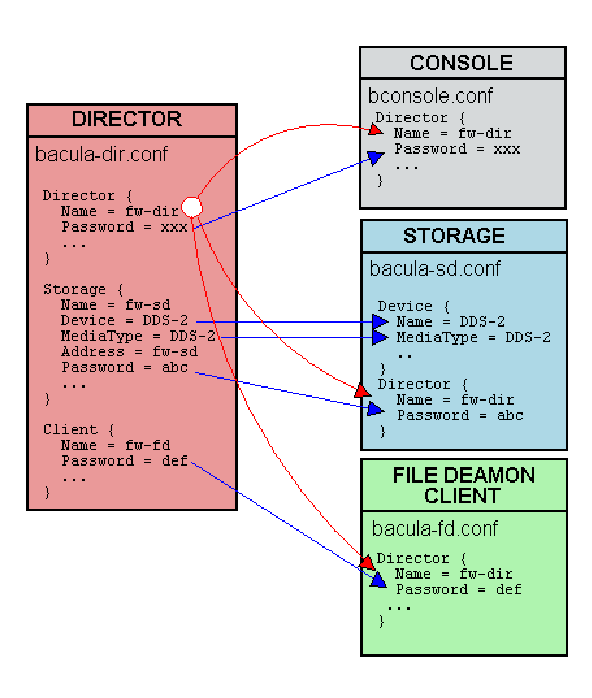
\includegraphics{./Conf-Diagram.eps} 

In the left column, you will find the Director, Storage, and Client resources,
with their names and passwords -- these are all in {\bf bacula-dir.conf}. In
the right column are where the corresponding values should be found in the
Console, Storage daemon (SD), and File daemon (FD) configuration files. 

Please note that the Address, {\bf fd-sd}, that appears in the Storage
resource of the Director, preceded with and asterisk in the above example, is
passed to the File daemon in symbolic form. The File daemon then resolves it
to an IP address. For this reason, you must use either an IP address or a
fully qualified name. A name such as {\bf localhost}, not being a fully
qualified name, will resolve in the File daemon to the localhost of the File
daemon, which is most likely not what is desired. The password used for the
File daemon to authorize with the Storage daemon is a temporary password
unique to each Job created by the daemons and is not specified in any .conf
file. 

\subsection*{Detailed Information for each Daemon}
\index[general]{Detailed Information for each Daemon }
\index[general]{Daemon!Detailed Information for each }
\addcontentsline{toc}{subsection}{Detailed Information for each Daemon}

The details of each Resource and the directives permitted therein are
described in the following chapters. 

The following configuration files must be defined: 

\begin{itemize}
\item 
   \ilink{Console}{_ChapterStart36} -- to define the resources for 
   the Console program (user interface to the Director).  It defines which
Directors are  available so that you may interact with them. 
\item 
   \ilink{Director}{_ChapterStart40} -- to define the resources 
   necessary for the Director. You define all the Clients  and Storage daemons
that you use in this configuration file.  
\item 
   \ilink{Client}{_ChapterStart25} -- to define the resources for 
   each client to be backed up. That is, you will have a separate  Client
resource file on each machine that runs a File daemon. 
\item 
   \ilink{Storage}{_ChapterStart31} -- to define the resources to 
   be used by each Storage daemon. Normally, you will have  a single Storage
daemon that controls your tape drive or tape  drives. However, if you have
tape drives on several machines,  you will have at least one Storage daemon
per machine.  
\end{itemize}
